\section{Results}

We report in this section results on standard examples, using both low and high
dimensional data. Unless specified otherwise, all the models were parameterized
using values given in table \ref{table:parameters}. These values were chosen to
be simple and do not really impact the performance of the model.
%%
\begin{table}[!ht]
  \begin{center}
    \begin{tabular}{ll}
        \textbf{Parameter} & \textbf{Value} \\
        \hline
        Number of epochs      ($t_f$)           & 25000\\
        Learning rate initial ($\varepsilon_i$) & 0.50\\
        Learning rate final   ($\varepsilon_f$) & 0.01\\
        Sigma initial         ($\sigma_i$)      & 0.50\\
        Sigma final           ($\sigma_f$)      & 0.01\\
    \end{tabular}
      \caption{\textbf{Default parameters} Unless specified otherwise, these are
        the parameters used in all the simulations.}
      \label{table:parameters}
  \end{center}
\end{table}
All simulations and figures were produced using the Python scientific stack,
namely, SciPy \citep{Jones:2001}, Matplotlib \citep{Hunter:2007} and
NumPy \citep{Walt:2011}. Sources are available at
\href{https://github.com/rougier/VSOM}{github.com/rougier/VSOM}.\\


\subsection{Low-dimensional data}

\subsubsection{One-dimensional data}

\begin{figure}
  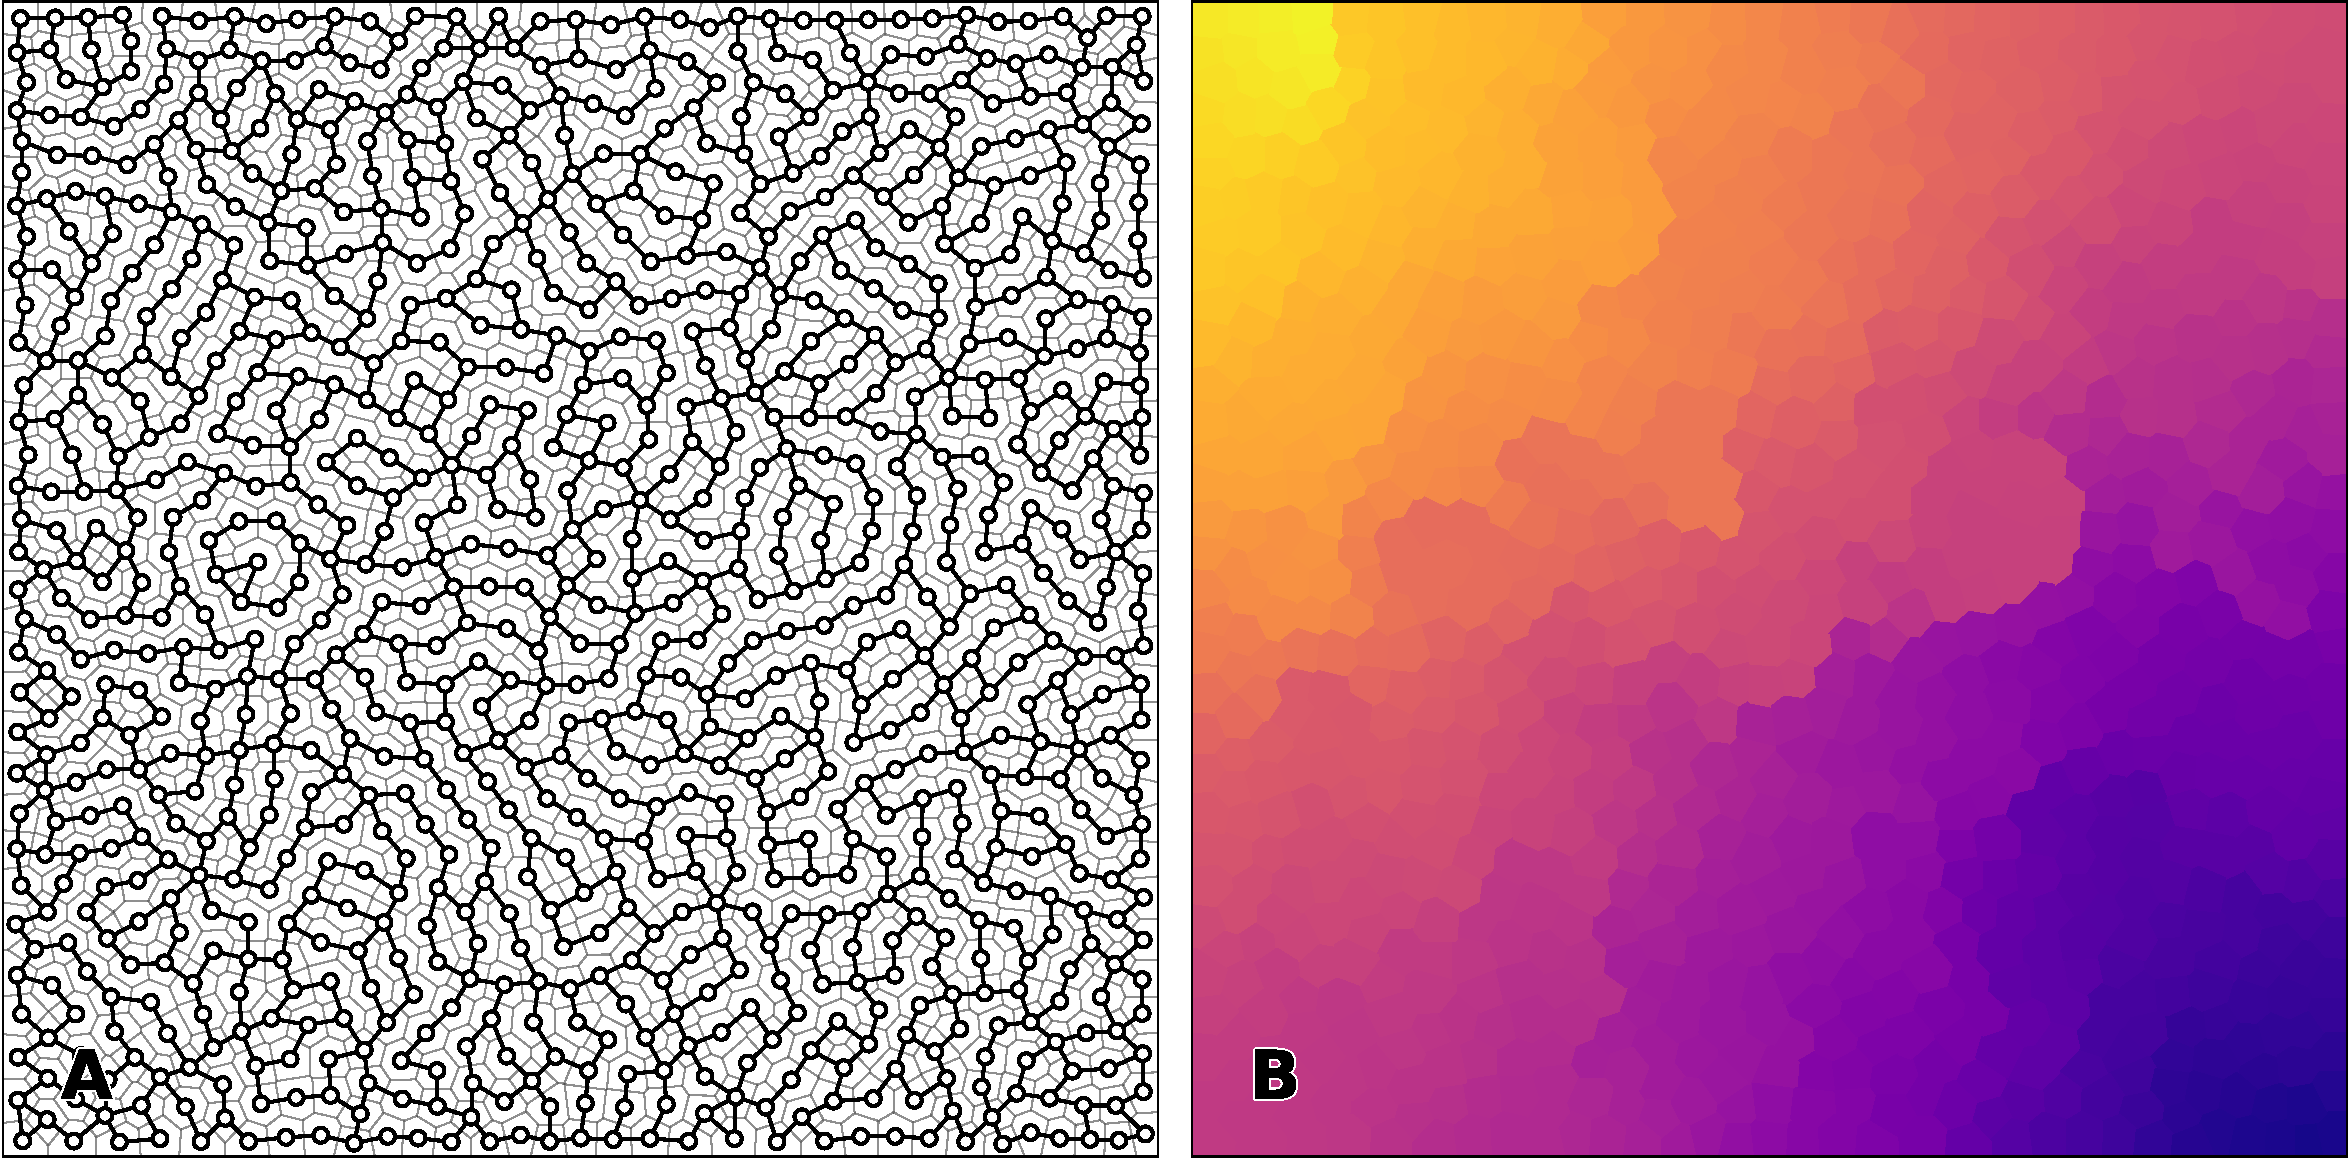
\includegraphics[width=\columnwidth]{figures/vsom-scalar-1.pdf}

  \vspace{2mm}
  
  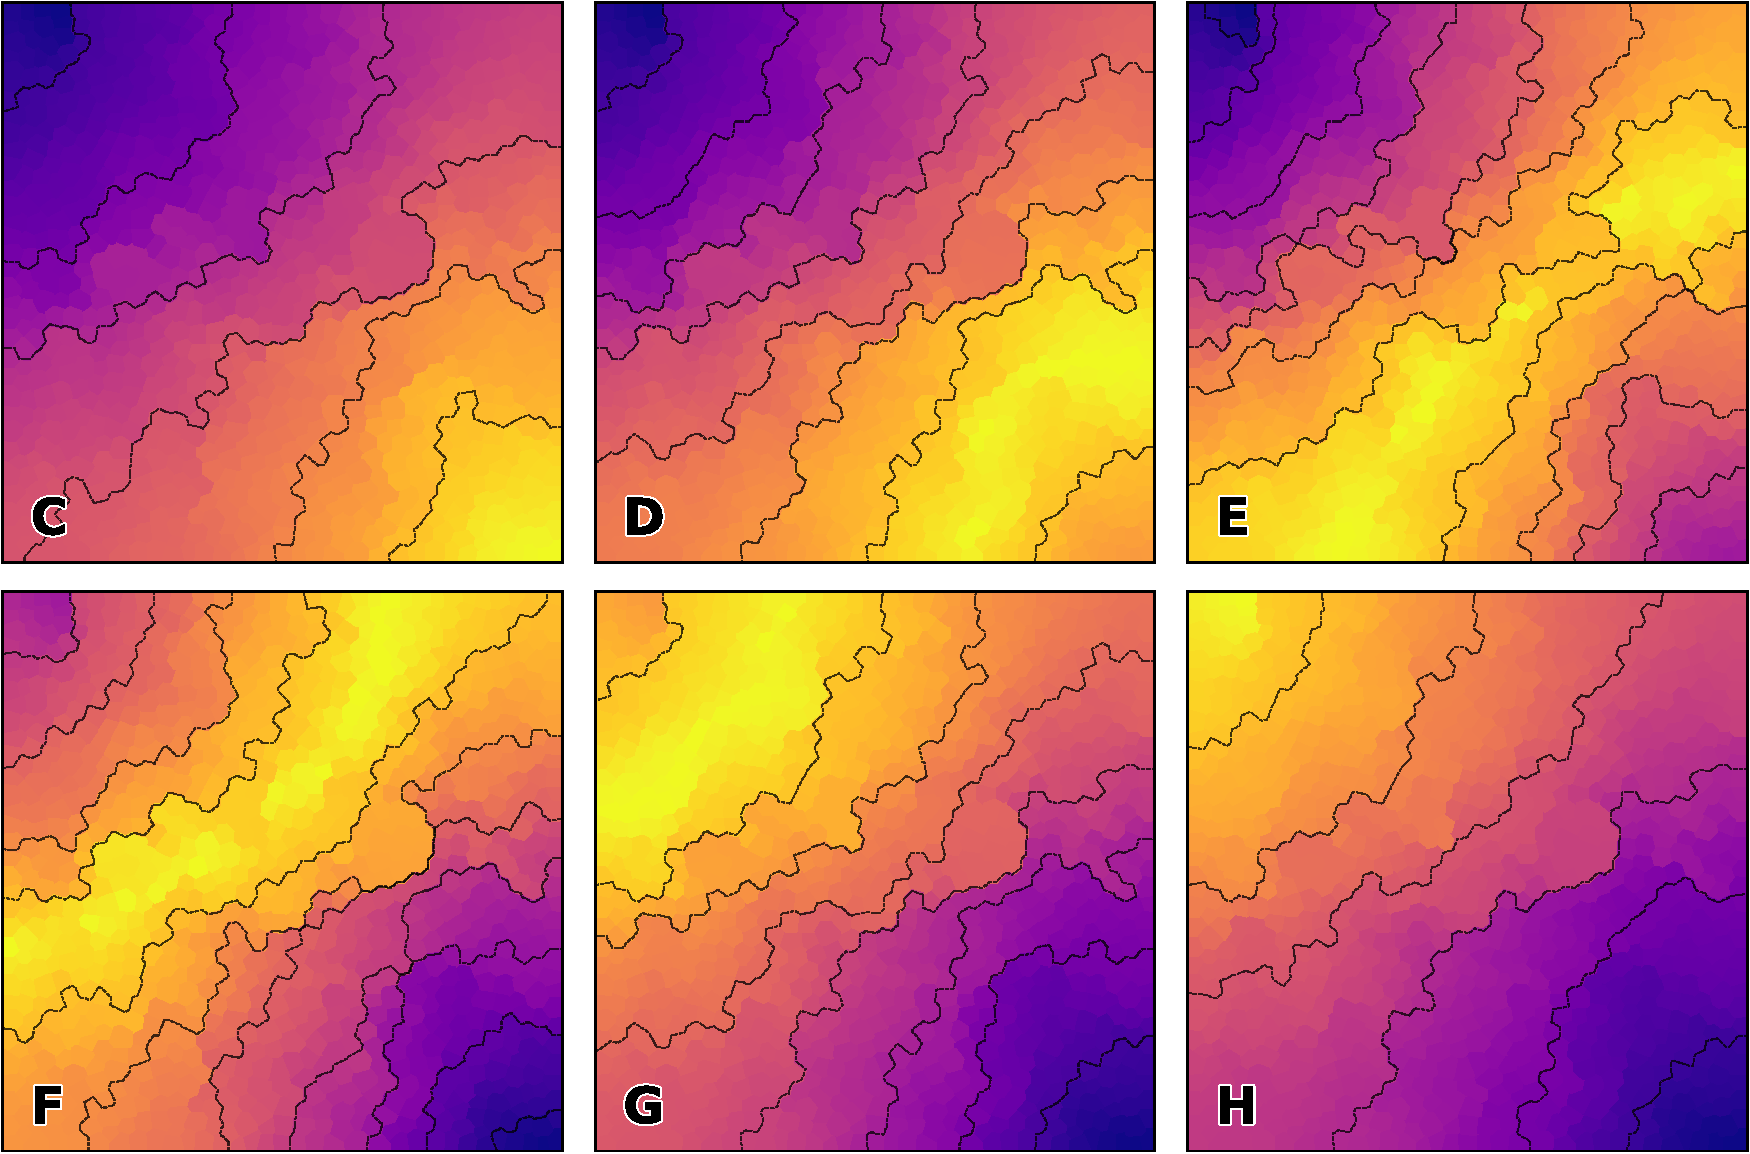
\includegraphics[width=\columnwidth]{figures/vsom-scalar-2.pdf}

  \vspace{2mm}
  
  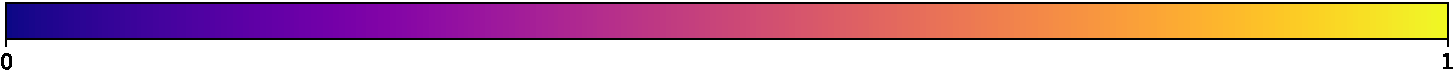
\includegraphics[width=\columnwidth]{figures/colormap.pdf}
  
  \caption{Voronoidal SOM made of 1003 neurons with a 2-nearest neighbors
    induced topology. Model has been trained for 10,000 epochs on random
    uniform scalars in [0,1]. \textbf{A} Map topology in the neural
    space. \textbf{B} Map prototypes displayed in neural space using Voronoi
    cells (whose color indicates prototype according to colormap). \textbf{C to
      H} Map activity for some random data (\textbf{C}:0.0, \textbf{D}:0.2,
    \textbf{E}: 0.4, \textbf{F}:0.6, \textbf{G}:0.8, \textbf{H}:1.0).}
\end{figure}

\begin{figure}
  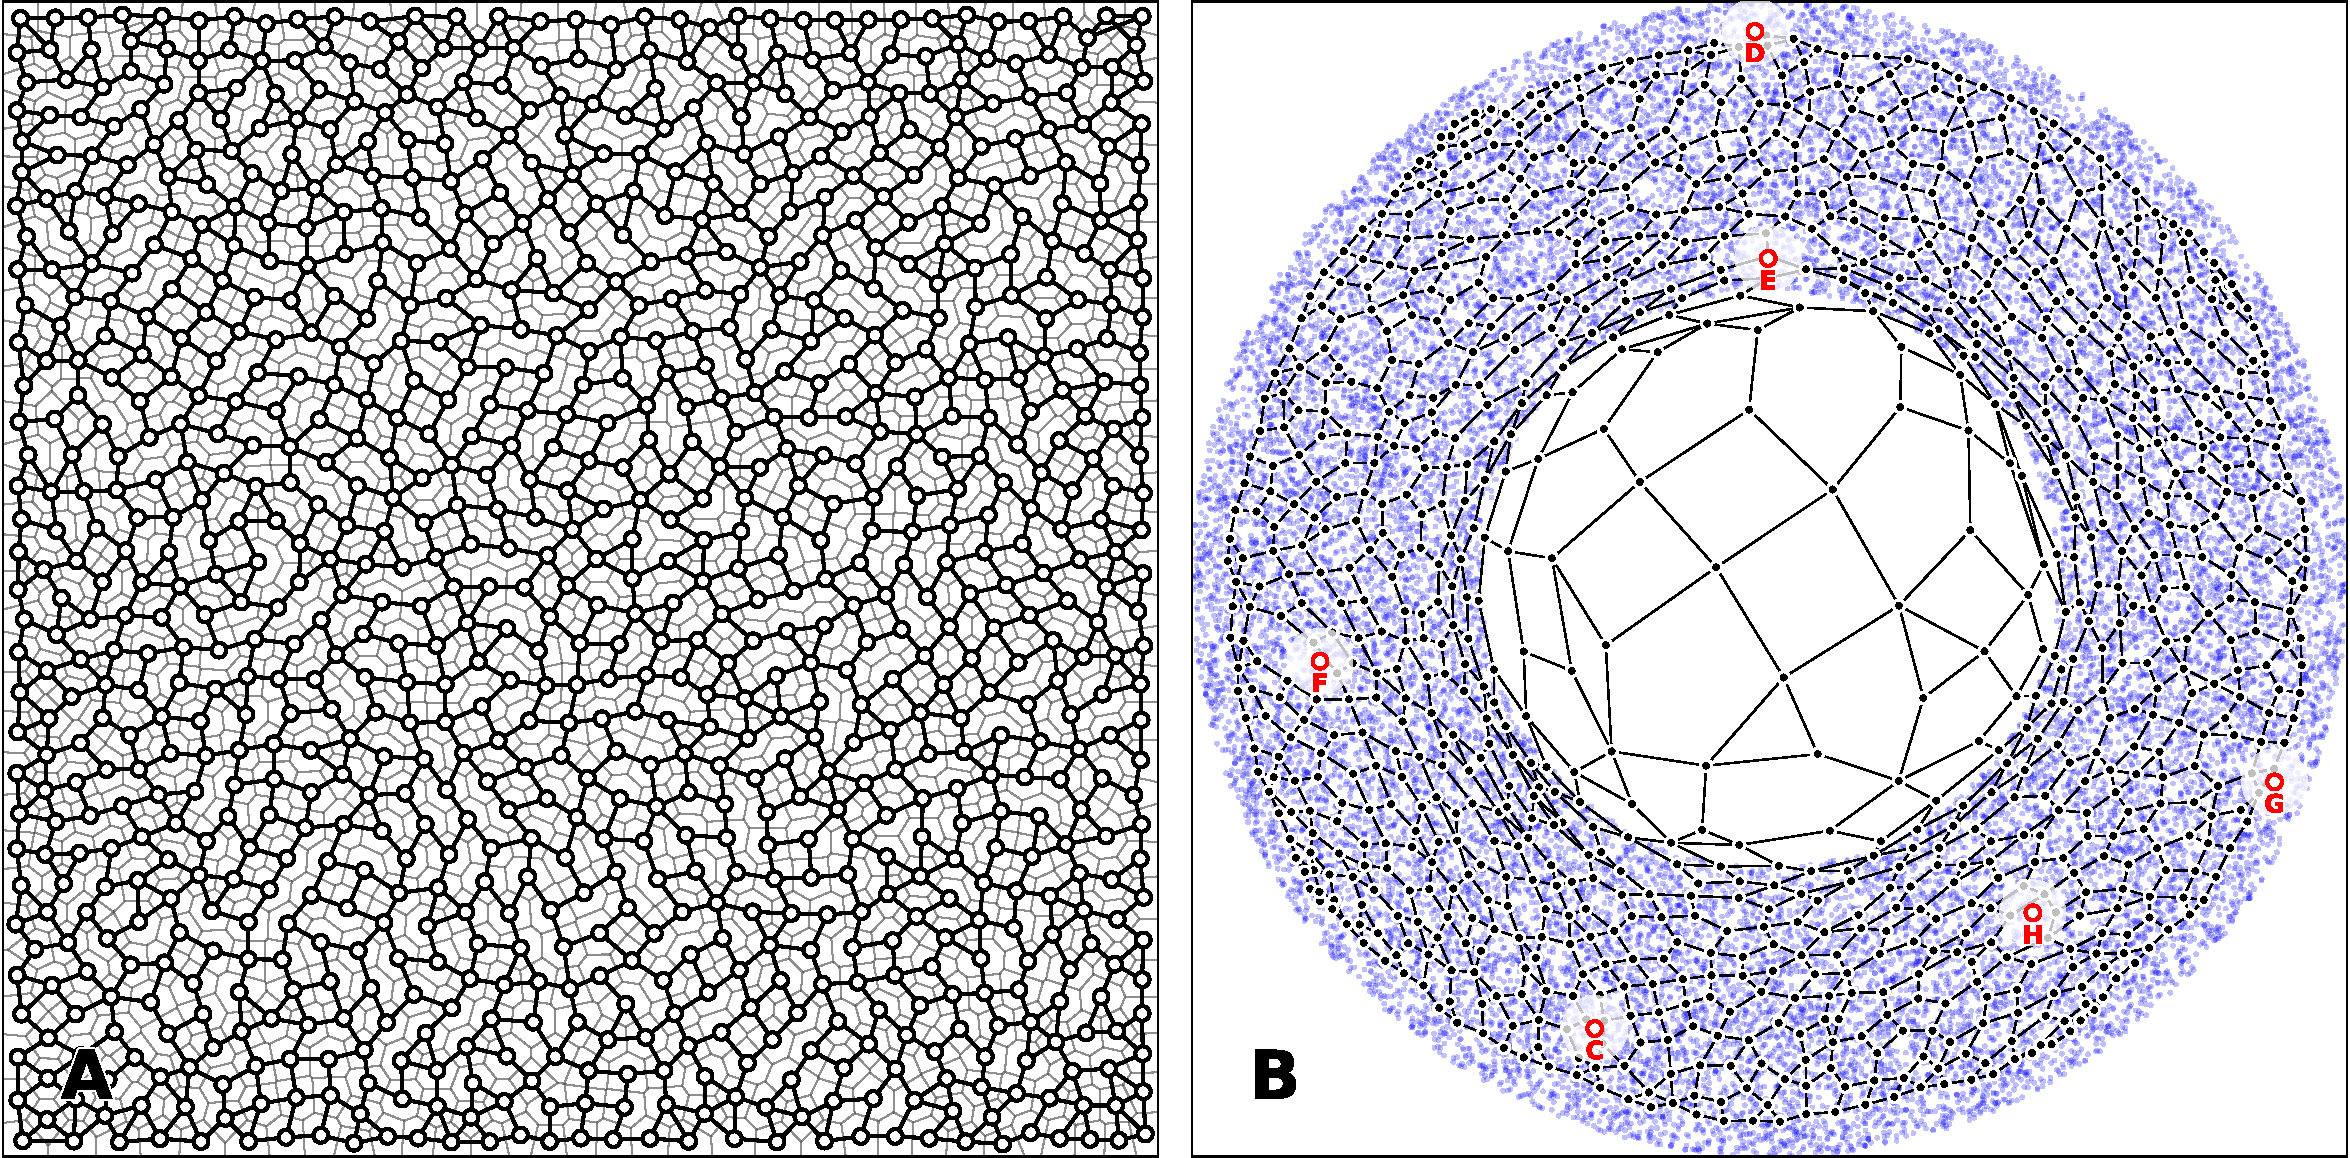
\includegraphics[width=\columnwidth]{figures/vsom-spatial-1.pdf}

  \vspace{2mm}
  
  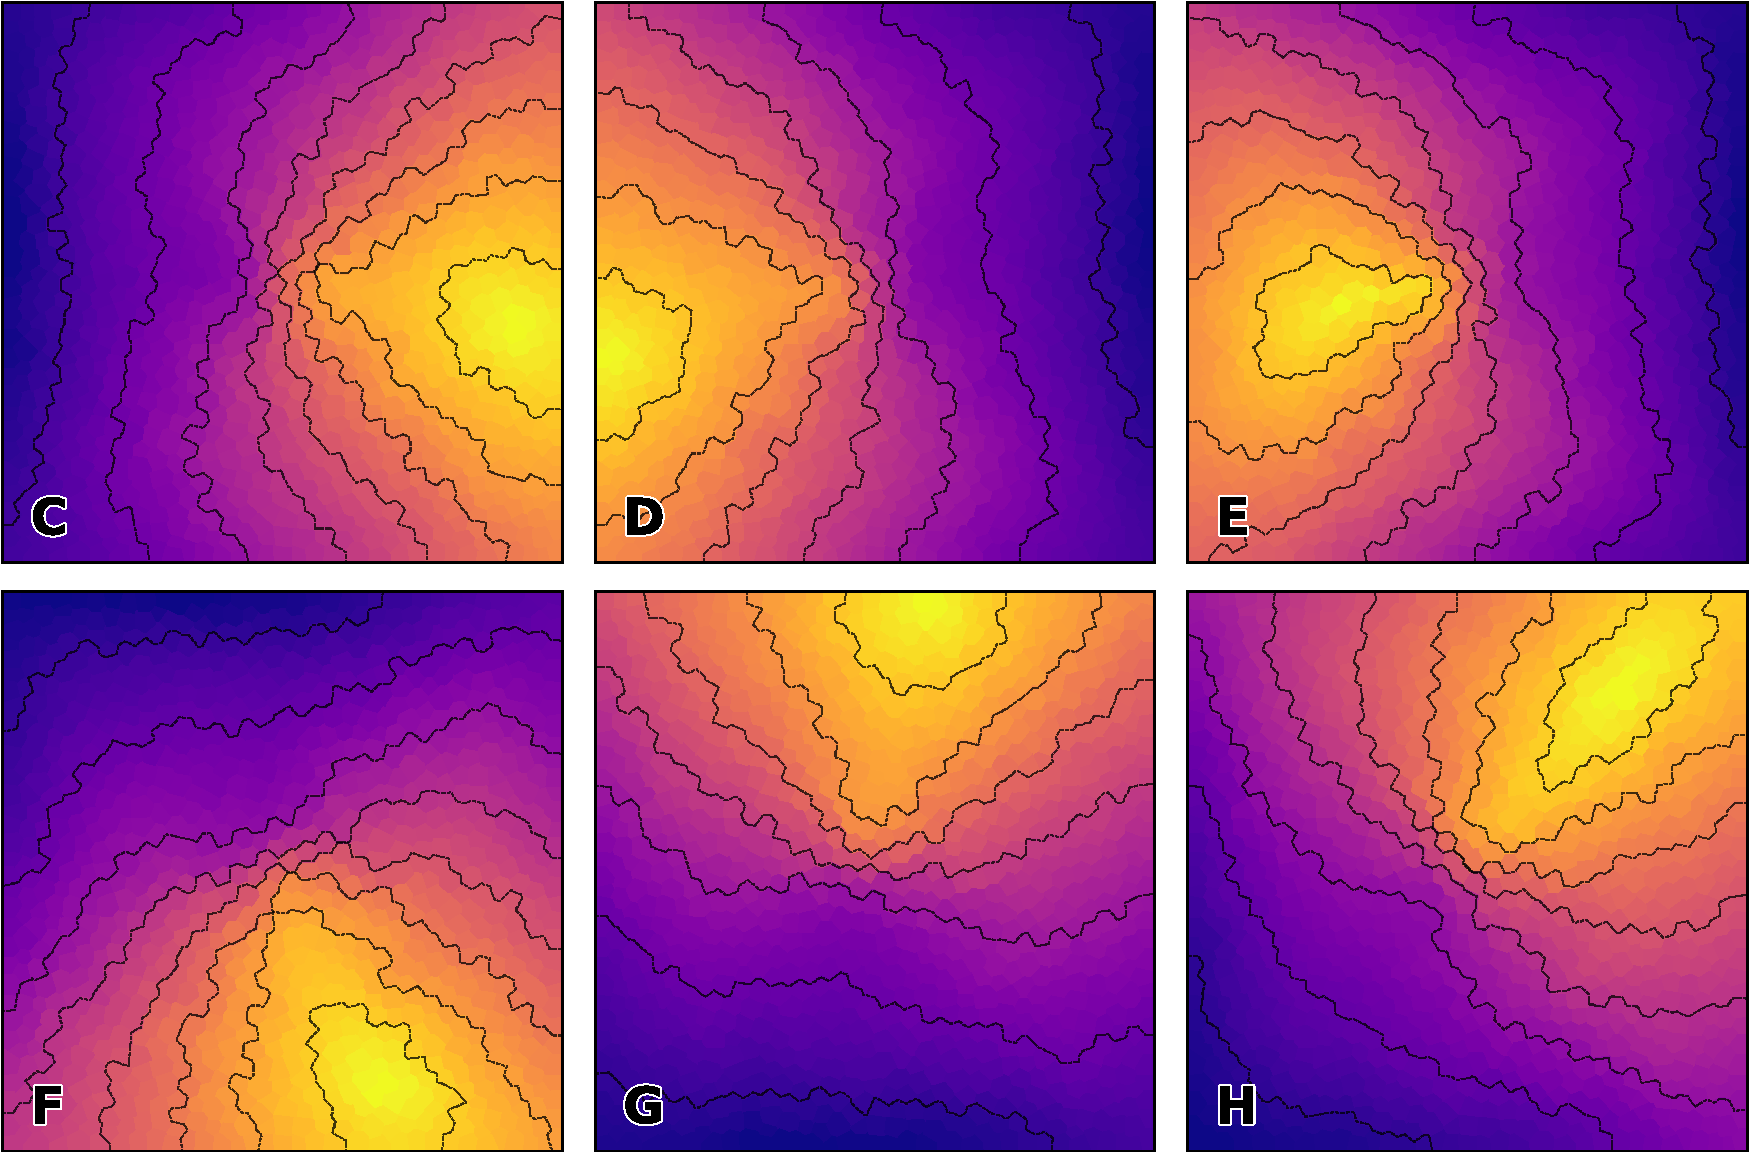
\includegraphics[width=\columnwidth]{figures/vsom-spatial-2.pdf}

  \vspace{2mm}

  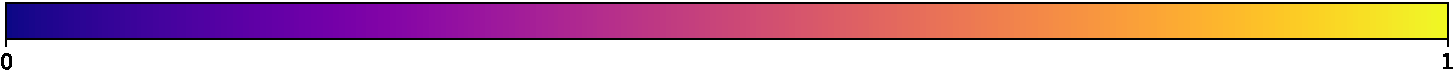
\includegraphics[width=\columnwidth]{figures/colormap.pdf}
  \caption{Voronoidal SOM made of 1003 neurons with a 3-nearest neighbors
    induced topology. Model has been trained for 25,000 epochs on random
    samples inside a torus. \textbf{A} Map topology in the neural
    space. \textbf{B} Map prototypes displayed in data space, blue points are
    the actual samples. \textbf{C to H} Map activity for some random data
    (shown on subplot \textbf{B}).}
\end{figure}

\begin{figure}
  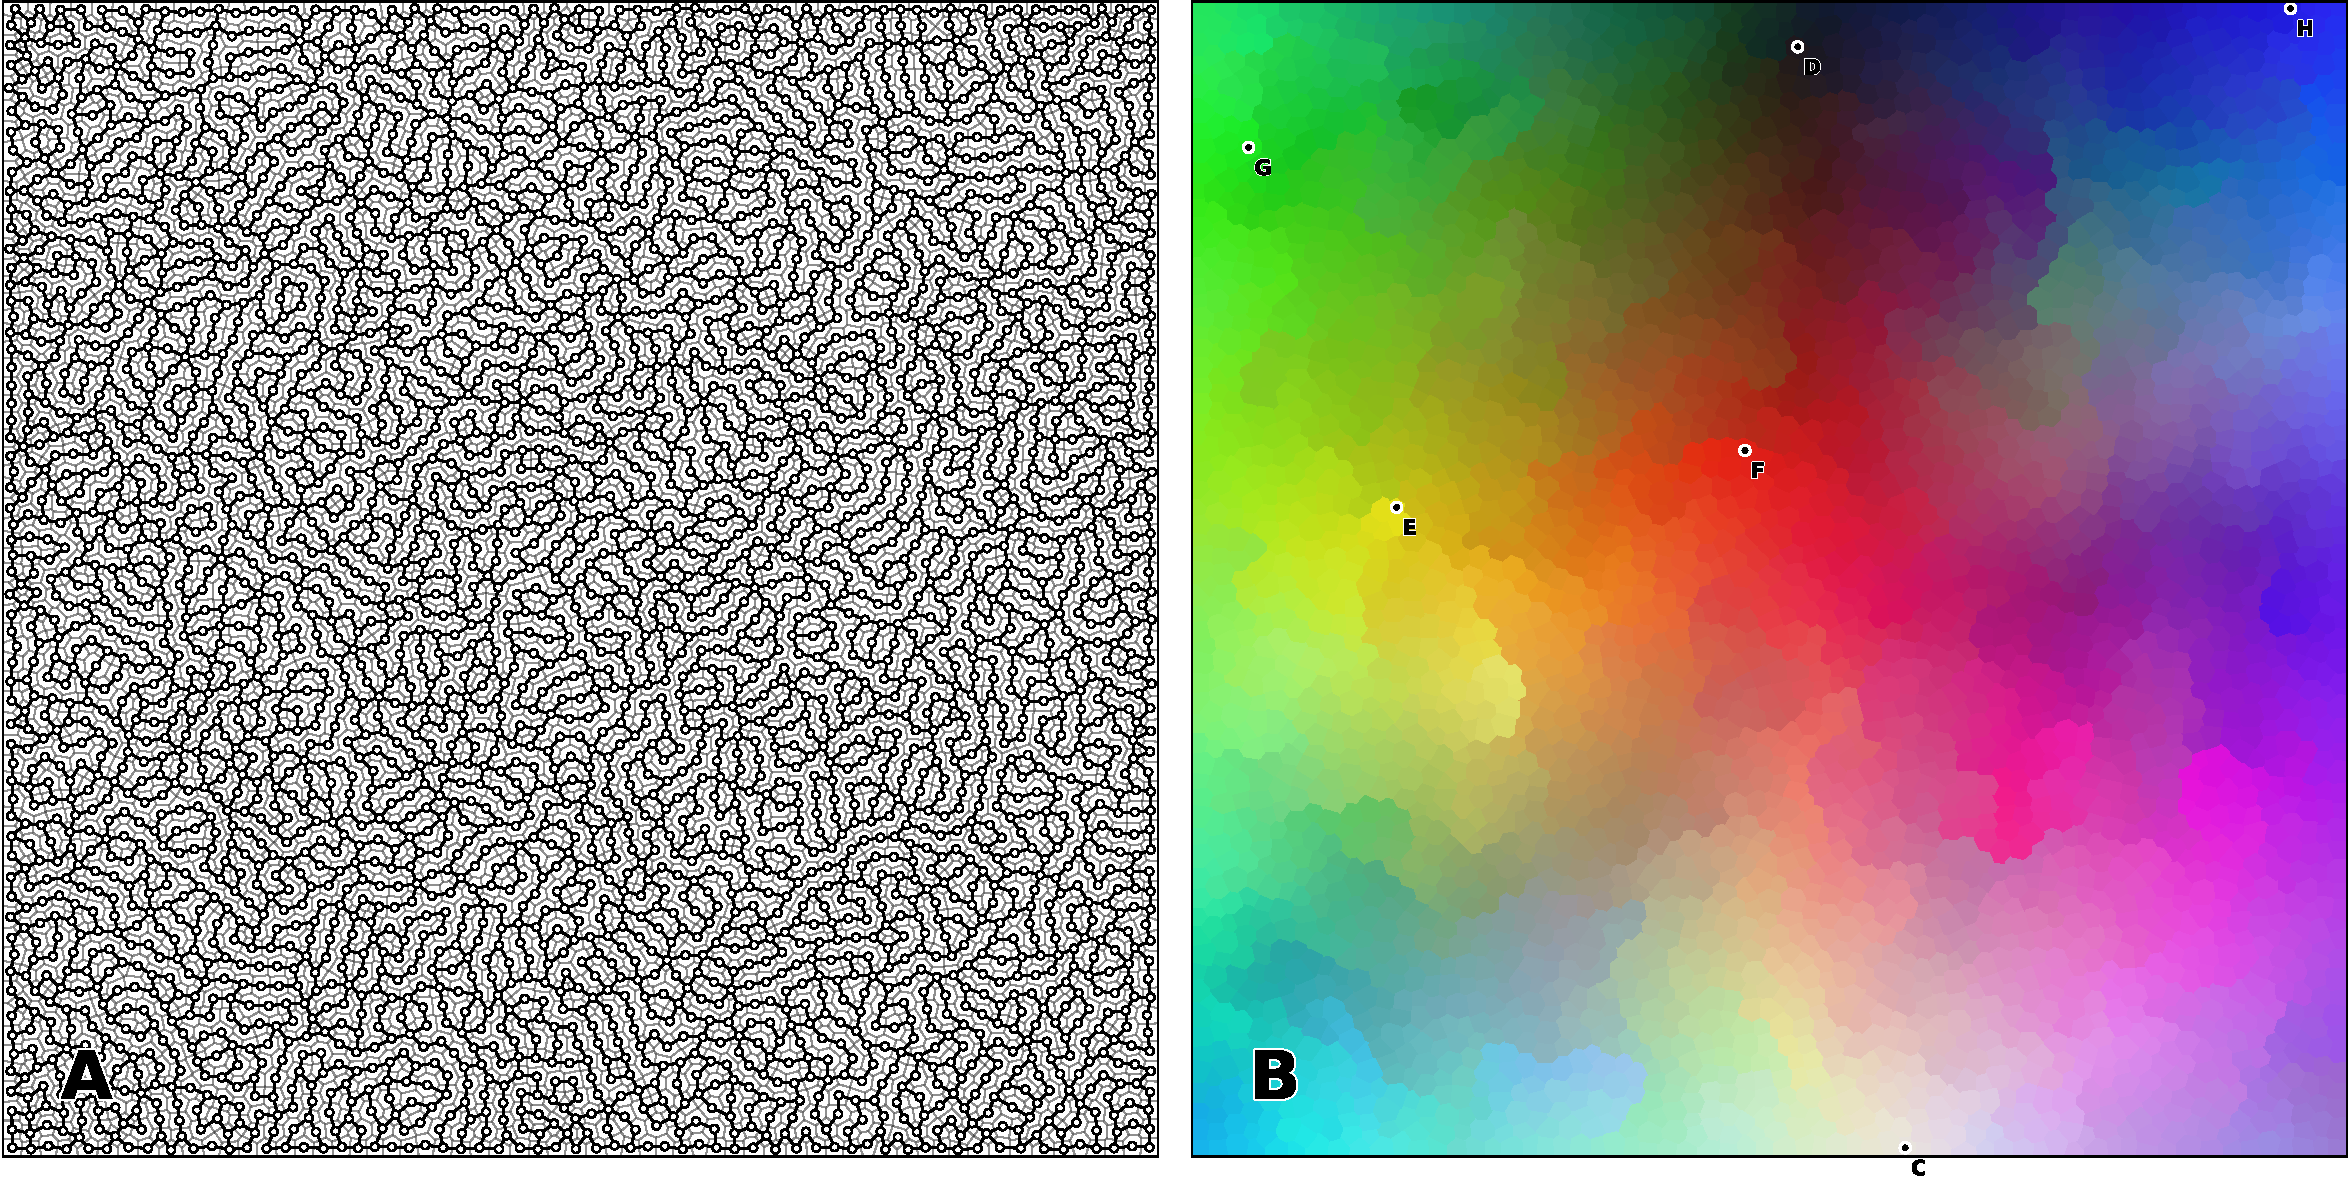
\includegraphics[width=\columnwidth]{figures/vsom-colors-1.pdf}

  \vspace{2mm}
  
  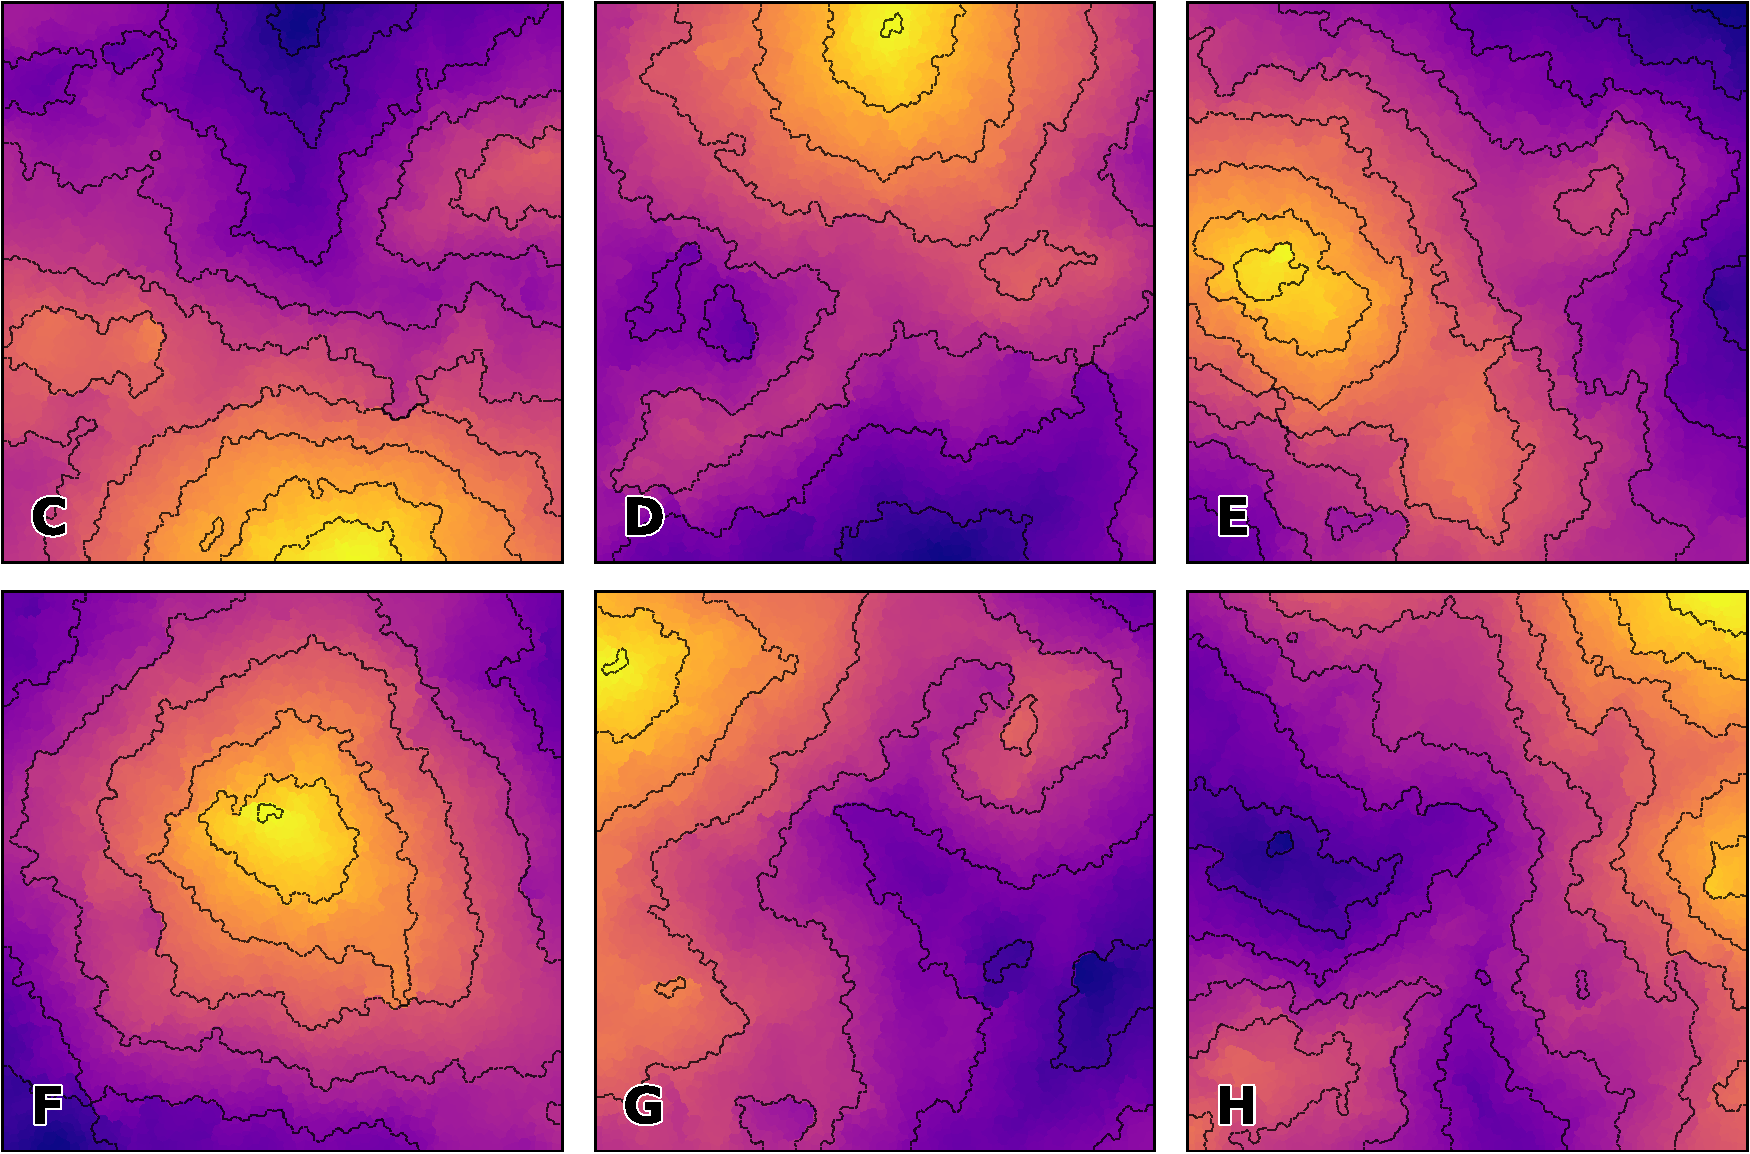
\includegraphics[width=\columnwidth]{figures/vsom-colors-2.pdf}

  \vspace{2mm}

  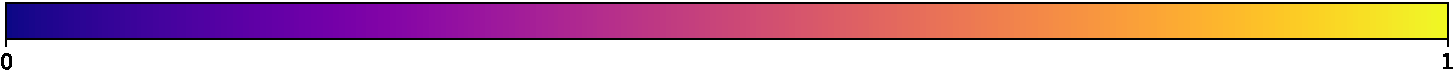
\includegraphics[width=\columnwidth]{figures/colormap.pdf}

  \caption{}
\end{figure}

\subsection{High-dimensional data}






\begin{figure}
  \setlength{\fboxsep}{0pt}%
  \setlength{\fboxrule}{.25pt}%

  \fbox{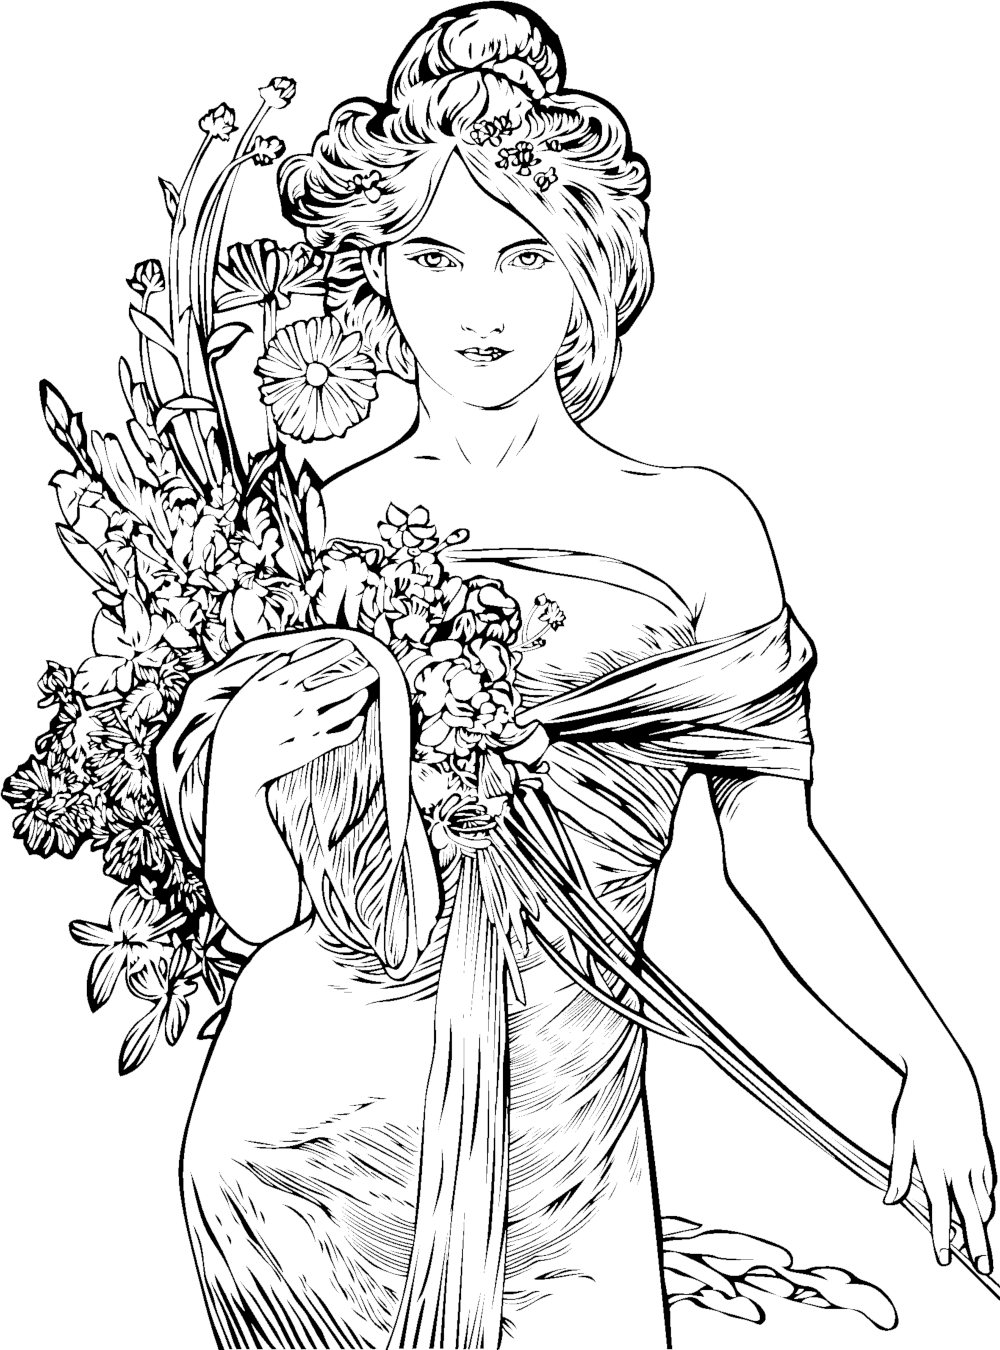
\includegraphics[height=5.1cm]{figures/mucha.png}}
        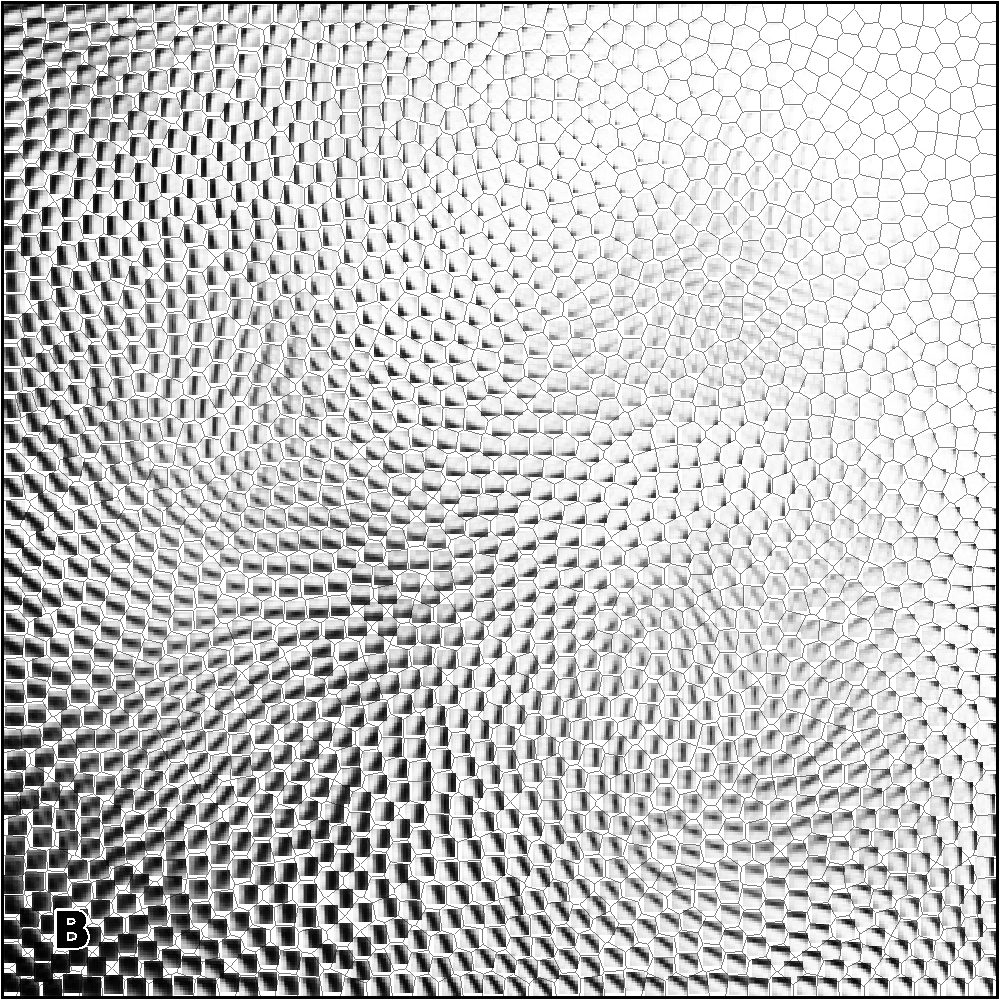
\includegraphics[height=5.1cm]{figures/vsom-image.pdf}
  \fbox{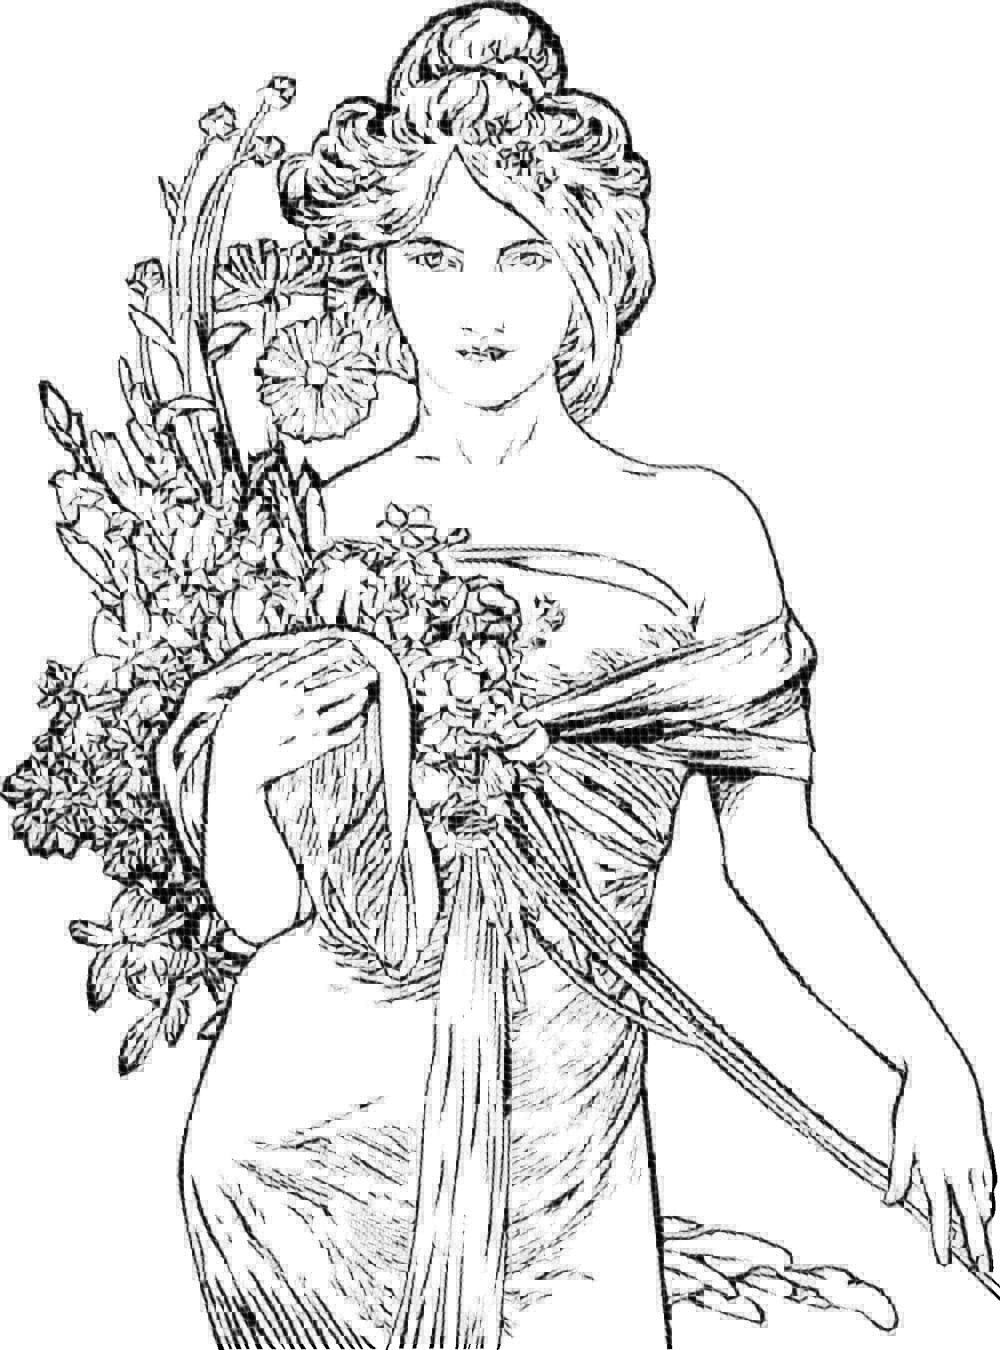
\includegraphics[height=5.1cm]{figures/mucha-vsom.png}}

%  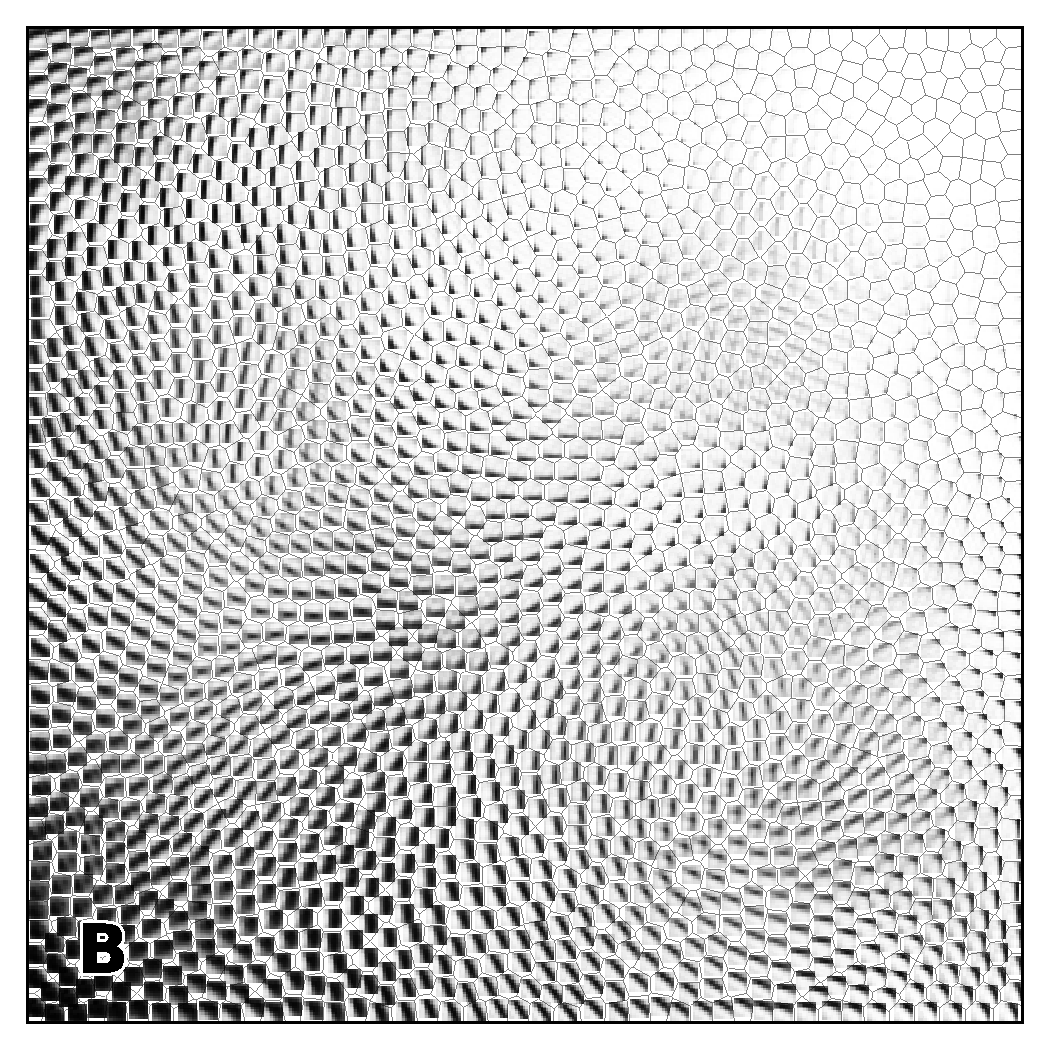
\includegraphics[width=\textwidth]{figures/vsom-image-1.pdf}
  
  \vspace{2mm}

  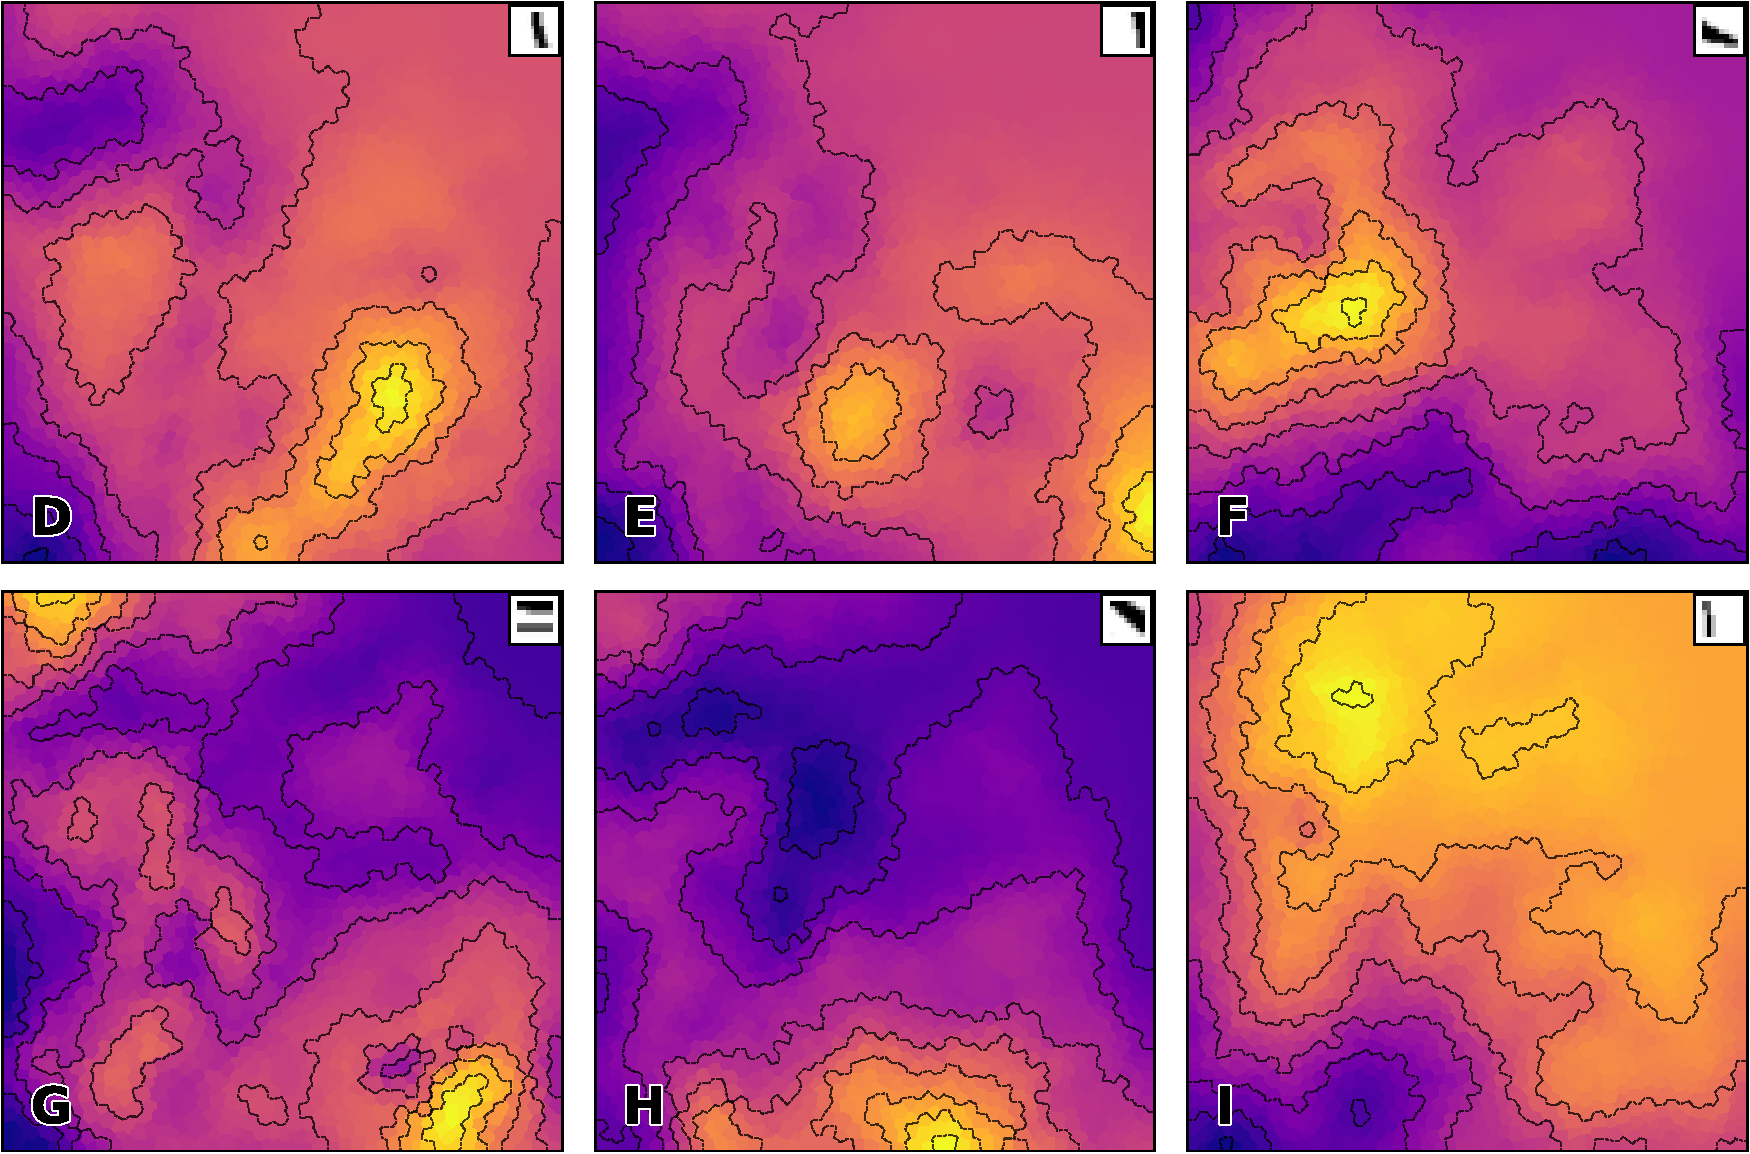
\includegraphics[width=\textwidth]{figures/vsom-image-2.pdf}

  \caption{Voronoidal SOM made of 1003 neurons with a 2-nearest neighbors
    induced topology. Model has been trained for 10,000 epochs on random
    uniform scalars in [0,1]. \textbf{A} Map topology in the neural
    space. \textbf{B} Map prototypes displayed in neural space using Voronoi
    cells (whose color indicates prototype according to colormap). \textbf{C to
      H} Map activity for some random data (\textbf{C}:0.0, \textbf{D}:0.2,
    \textbf{E}: 0.4, \textbf{F}:0.6, \textbf{G}:0.8, \textbf{H}:1.0).}
\end{figure}


\subsection{Reorganization}
